\documentclass{mcmthesis}
\mcmsetup{CTeX = false,   % enable Chinese character 使用 CTeX 套装时,设置为 true
        tcn = 00000000, problem = D,
        sheet = true, titleinsheet = true, keywordsinsheet = true,
        titlepage = false, abstract = false}
\title{}
\date{\today}

\usepackage{indentfirst} % 首行自动缩进

\usepackage{subfiles} % Best loaded last in the preamble
\usepackage{array}
\usepackage{tabularx}
\usepackage{listings}
\usepackage{amsmath}
\usepackage{subcaption}
\usepackage{titlesec}
\usepackage{setspace}

\begin{document}

\setlength{\parskip}{0.1\baselineskip}
\begin{spacing}{1}
  %%行间距变为double-space
  \subfile{sections/abstract}
\end{spacing} 


\begin{spacing}{1}

% Generate the Table of Contents if it's needed.
\tableofcontents
\newpage


% Generate the Memorandum, if it's needed.
% \memoto{\LaTeX{}studio}
% \memofrom{Liam Huang}
% \memosubject{Happy \TeX{}ing!}
% \memodate{\today}
% \logo{\LARGE I'm pretending to be a LOGO!}
% \begin{memo}[Memorandum]
%   ;
% \end{memo}


\section{Introduction}

\graphicspath{{figures/}{../figures/}}

\subsection{Background}
Wildfire spreads rapidly in Australia. 
In fire season, it's devastating for people's safety and properties. Victoria's
Country Fire Authority (CFA) uses different means to protect its people. 
Drones carrying high definition \& thermal imaging cameras and telemetry 
sensors were sent for surveillance and situational awareness (SSA). 
Drone repeaters, transceivers that automatically rebroadcast signals 
at higher powers can help connect Emergency Operations Center (EOC) with SSA and front-line employees with VHF/UHF bands.

\subsection{Problem Restatement}

\subsubsection{Limits}

\begin{itemize}
  \item
    Drone-related
  
    \begin{itemize}
    \item
      Cost \$1000 per drone
    \item
      Flight Range 30 km
    \item
      Transmission Range 20 km
    \item
      Flight Speed 20 m/s
    \end{itemize}
  \item
    Fire-related
  
    \begin{itemize}
    \item
      Size
    \item
      Frequency
    \end{itemize}
  \end{itemize}

\subsubsection{Targets}


\begin{itemize}
  \item
    Deployment of drones for fast response
  
    \begin{itemize}
    \item
      Reduce cost
    \item
      Increase weighted coverage
    \end{itemize}
  \item
    Fire Prediction
  \item
    Deployment of drones for front-line personnel in different
    circumstances
  
    \begin{itemize}
    \item
      Build models for different fire size
    \item
      Build models considering different terrians
    \end{itemize}
  \end{itemize}

\subsection{Our Work}
\begin{figure}[h!]
  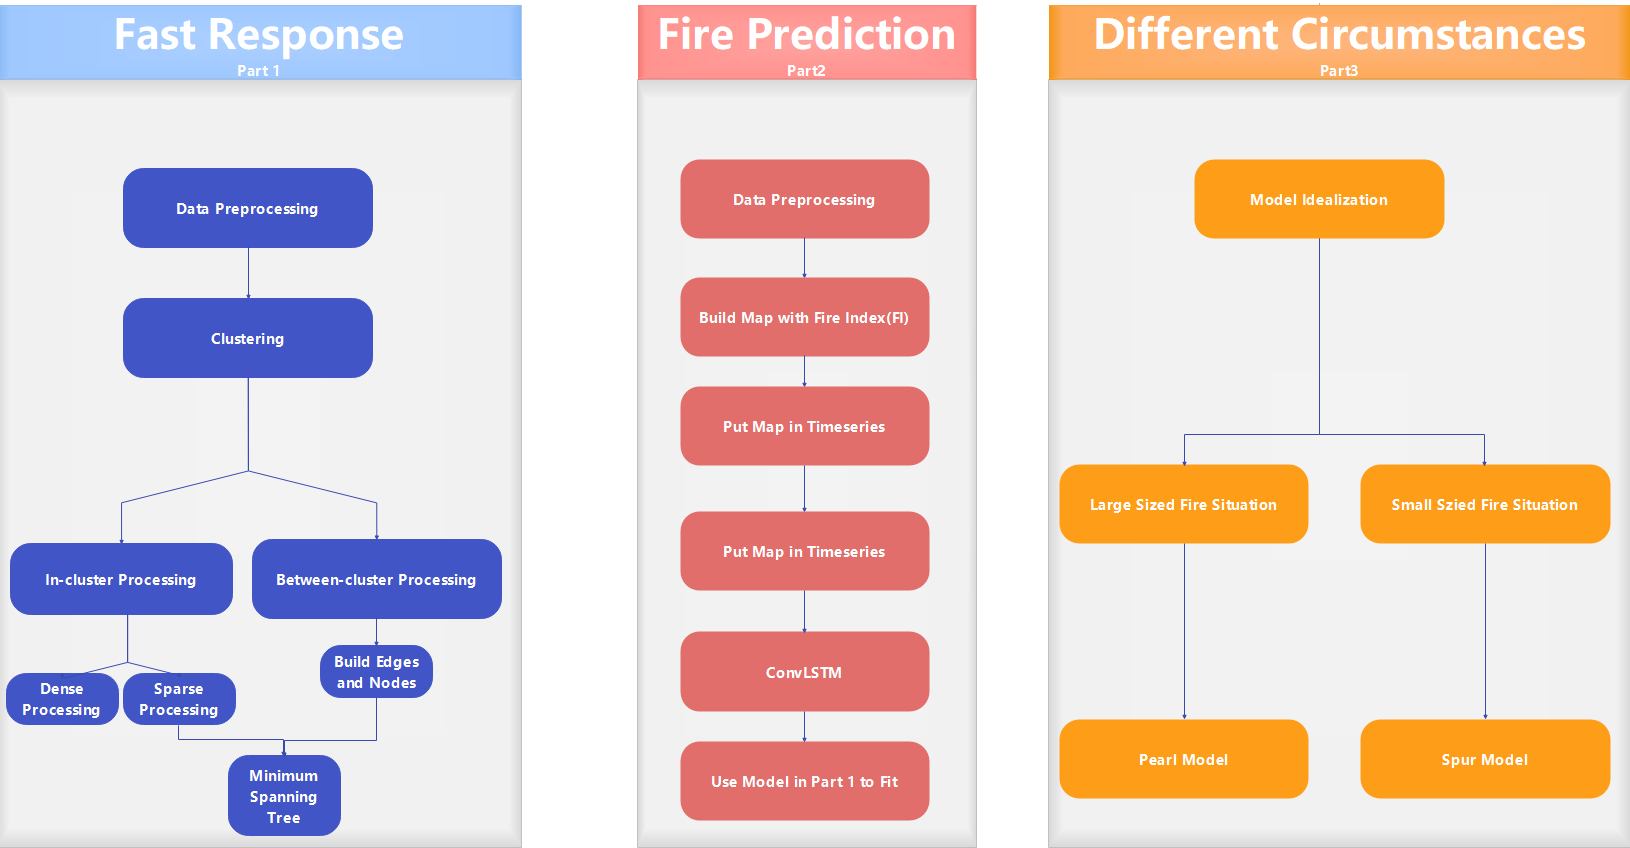
\includegraphics[width=\linewidth]{flowchart1.png}
  \caption{Our Work}
  % \label{fig:boat1}
\end{figure}

\section{List Of Symbols}
  \subfile{sections/symbols}

\section{General Assumptions}
  \subfile{sections/assumptions}

\section{The Models}
  \subfile{sections/models}

\section{Conclusions}
  \subfile{sections/conclusions}

\section{Model Evaluation And Improvement}
  \subfile{sections/evaluation}


\newpage
\end{spacing} 
\bibliographystyle{plain}
\bibliography{../reference/reference}




\end{document}
